\secrel{Расчет схем и моделирование в \ngs}\label{spice}\secdown
% \secdown

на основе статьи

\cp{http://www.mithatkonar.com/wiki/doku.php/kicad/kicad\_spice\_quick\_guide}

\cp{http://physics.gmu.edu/~rubinp/courses/407/ngspice.pdf}

Electronic circuit simulation with gEDA and NG-Spice by Example

\copyright\ Andreas Fester

\bigskip

\prog{\spice}: [S]imulation [P]rogram with [I]ntegrated [C]ircuit
[E]mphasis\ --- пакет программ симуляции и расчета электронных схем,
была создана для моделирования \emph{интегральных микросхем}, расчета режимов
работы, оптимизаии, и предсказания поведения.

\bigskip
\spice\ может выполнять несколько видо схемотехнических расчетов, самые важные
из которых:

\begin{itemize}
  \item
Нелинейный анализ по постоянному току: вычисление передаточной характеристики по
постоянному току
  \item
Нелинейный анализ переходных процессов: вычисление токов и напряжений как
функции времени в условиях большого сигнала
  \item
Линейный AC анализ: вычисление выхода как функции от частоты. Выводится
\term{bode plot}
  \item
Анализ шума
  \item
Расчет чувствительности
  \item
Анализ искажений
  \item
Фурье-анализ: вычисление и отображение частотных спектров
  \item
Анализ Монте-Карло
\end{itemize}

\bigskip

\secrel{Доступные SPICE-пакеты}\secdown

Первоначально \spice\ был разработан в Университете Беркли. Другие версии
\spice\ являются форками этой реализации, и сейчас существует несколько
вариантов:

\begin{itemize}
\item \href{http://ngspice.sourceforge.net/}{\ngs}: самый доступный
бесплатный OpenSource SPICE-движок.
\item \url{http://www.ngspice.com/}\ --- on-line вариант \prog{ngspice}, удобен
для начального обучения
\item \href{http://www.linear.com/designtools/software/}{\lts}:
Популярная бесплатная коммерческая версия от Linear Technology для \win.
Работает в \prog{WINE}. Поставляется в комплекте с графической оболочкой,
но требуется проверка файлов расчетных заданий, которые она создает.
\item
\href{https://www.gnu.org/software/gnucap/}{gnucap}\note{уже включен в
виндозную сборку KiCAD}:
Не совсем SPICE, но пытается быть синтаксически совместмой.
\item \href{http://www.spiceopus.si/}{SpiceOpus}: Коммерческая, но
удобная, особенно в плане вывода графиков.
\item
\href{http://www.cadence.com/products/orcad/pspice_simulation/Pages/default.aspx}{PSpice}:
\win-only, дорогой коммерческий пакет, стандарт de-facto для
профессионального применения в USA в составе тяжелых EDA-продуктов.
Они традиционно предоставляют обрезанную \emph{gratis}-версию для студентов.
Также имеет в комплекте GUI.
\item \prog{MultiSim}, \prog{OrCAD}, \prog{DesignLab},.. коммерческие
EDA-пакеты, содержит в составе одну из версий \prog{P\spice}
\item Какие-то еще?
\end{itemize}

В этом разделе описан \ngs, который был написан с целью полностью переписать
оригинальную реализацию Беркли \spice. Сейчас он все еще содержчит часть кода
Беркли, но в этом коде было исправлено множество ошибок.
Важно пониать, что каждая реализация \spice\ может вести себя особенно в
некоторых случаях: некоторые из них более совместимы между собой, другие менее.
Всегда важно прочитать документацию, которая поставляется с конкретной
версией \spice. Дистрибутив \ngs\ пославляется с детальным руководством
пользователя, а этот раздел поможет вам начать. Хорошо иметь под рукой полное
руководство при чтении этого раздела, так как интересующие вас команды там
рассмотрены детальнее.

\secrel{Установка \ngs\ под \win}

\menu{\winr\url{http://ngspice.sourceforge.net/download.html}>\prog{ng-spice-rework}>\file{ngspice-xx\_xxxxxx.zip}}

\menu{unzip \file{ngspice-xx\_xxxxxx.zip}>\file{C:/spice}}

\menu{\winstart>Компьютер>\rms>Свойства>Дополнительные
параметры системы}

\menu{Переменные среды>\file{PATH=\ldots;C:/spice/bin}}

\secrel{Установка \lts\ (только \win)}

\menu{\winr>\url{http://www.linear.com/designtools/software/}}

\secrel{Установка \ngs\ под \linux}

\begin{verbatim}
root# aptitude install ngspice
\end{verbatim}

Пакет \pack{\ngs}\ также может быть легко собран и установлен компиляцией
их исходниов. После загрузки архива, соберите пакет для вашего дистрибутива:
\begin{verbatim}
tar xvzf ng-spice-rework-15.tgz
 cd ng-spice-rework-15
./configure --with-readline=yes
make
checkinstall
\end{verbatim}

Убедитесь что в системе присутствует библиотека \pack{GNU readline}, и она
включена в опциях \prog{configure}: ее использование делает интерфейс командной
строки более комфортным. Подробнее сборка \ngs\ описана в его руководстве в
составе дистрибутива.

\bigskip
Сборка \ngs\ для az\linux\ описана в разделе \ref{azspice}.

\secup

\secrel{Пошаговый пример использования}

Рассмотрим очень простой пример симуляции электронной схемы. В основном вы
будете рисовать ваши схемы в \eeschema, но интерактивная симуляция пока не
реализована.

\secdown

\secrel{Рисуем схему в \kicad}

Схема, которую мы хотим рассчитать\ --- простой \term{RC-фильтр}. Эта схема была
выбрана, так как она содержит очень ограниченное количетво элементов, и поэтому
понятна: источник напряжения, резистор и конденсатор. Использование редактора
схем вам уже должно быть знакомо из предыдущего раздела (\ref{eeschema}).
Запустите \eeschema\ и нарисуйте схему:

\bigskip
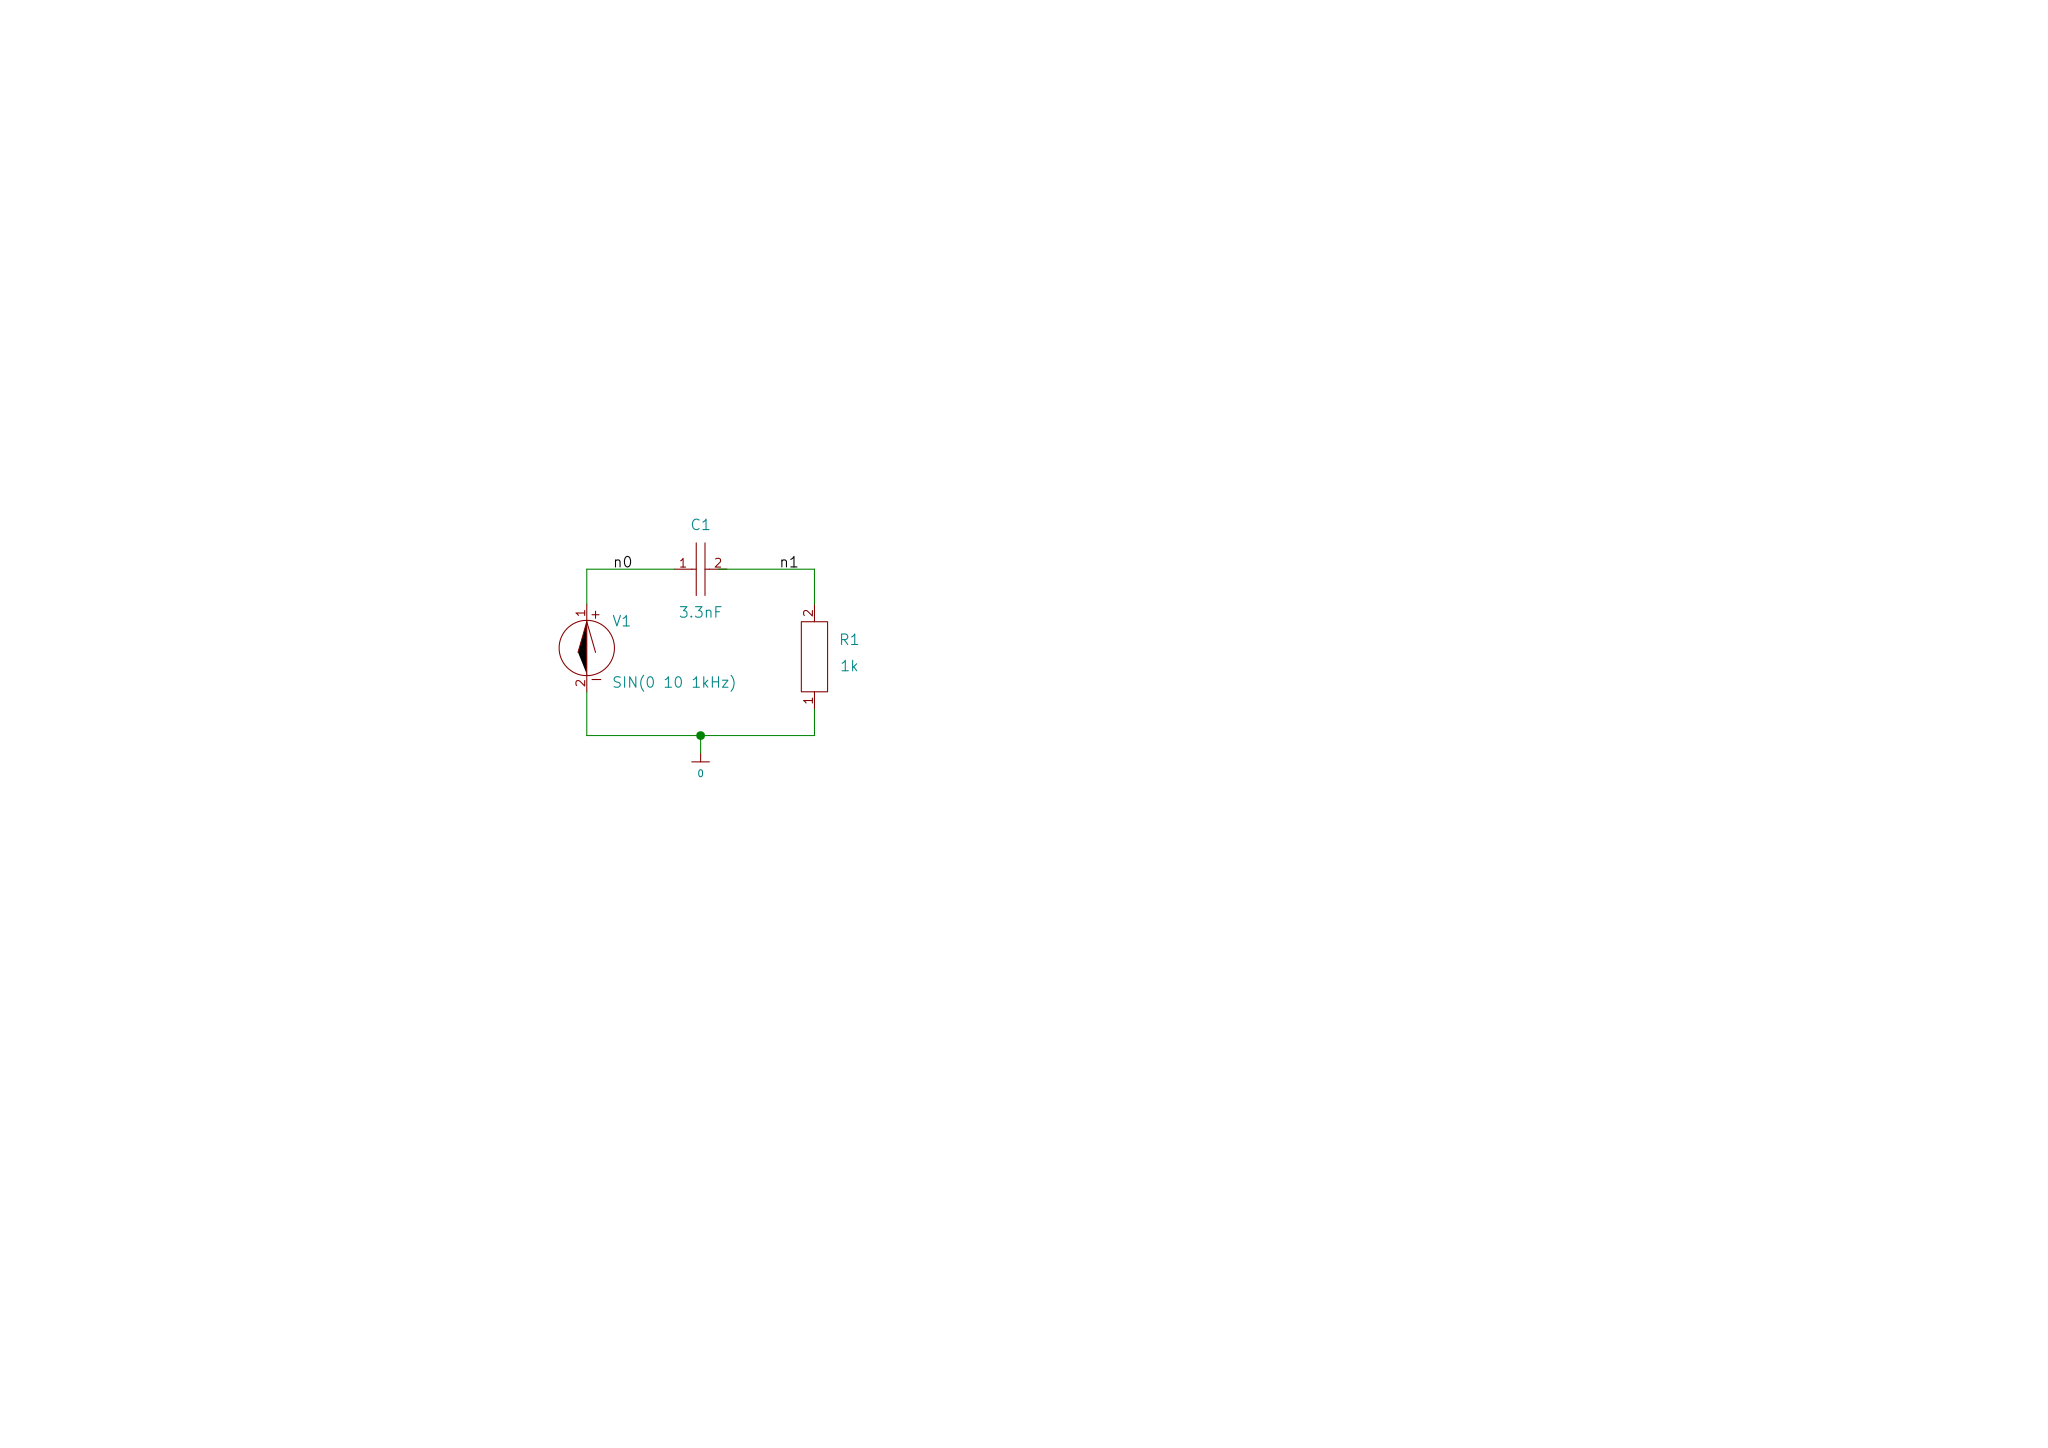
\includegraphics[height=0.5\textheight]{spice/RCfilter.pdf}
\fig{figspicerc}{Простой RC-фильтр}
\bigskip

Имена, указанные на проводниках\ --- \emph{имена цепей}. Они могут не
указываться, если вам не нужно на них ссылаться в расчете. При экспорте списка
цепей из \eeschema\ им будут присвоены униальные имена. Цепь может иметь любое
имя, за некоторым исключением: \emph{в списке должна быть одна цепь с именем
[\elem{0}], она подключается к общему проводу (земле)}. Рисуя схему, поместите
на нее один или несколько элементов [\elem{0}]\ из библиотеки \file{spice}.

\elem{V1}\ --- \term{независимый источник напряжения}. Его значение задано в
виде выражения \verb|SIN(0 10 1kHz)|, создающего синусоидальный (SIN) сигнал со
смещением (0)\,вольт, амплитудой (10)\,вольт и частотой (1kHz).

\bigskip
Рисуйте вашу схему, соблюдая несколько рекомендаций:
\begin{itemize}
  \item
Для именованных цепей используйте \emph{глобальные метки} вместо локальных.
В списке цепей глобальные идентификаторы цепей включаются как есть, а
локальные метки модифицируются, что делает сложным последующие ссылки на них при
SPICE-моделировании.
  \item
Используйте компонент [\elem{0}] из библиотеки \file{spice}, вместо обычного
комопнента [\elem{GND}]: ”\elem{0}” официальное имя главной земли в файлах
P\spice. Некоторые \spice-движки умеют транслировать $GND \rightarrow 0$, другие
нет.
\end{itemize}

\secrel{Создание списка цепей}

Входными данными для симуляции является \term{список цепей (netlist)}.
Список цепей создается через экспорт из \eeschema. Если
вы используете программу рисования схем, посмотрите в ее документации, умеет ли
она экспорт в \spice (\file{.cir}), и как это сделать.

\begin{itemize}
  \item
Кликните кнопку или пункт меню \menu{Сформирвать список цепей}.
  \item
Выберите вкладку \menu{Spice}, и убедитесь что включен крыжик \menu{\checkbox\
Формат по умолчанию}. Вам нужно сделать это только один раз, настройки
запоминаются.
\item
Нажмите кнопку \menu{Сформировать}
\end{itemize}

Если вы хотите запускать \ngs\ из диалога экспорта:
\begin{itemize}
  \item
Заполните полный путь с программе симуляции, типа
\file{C:/spice/bin/ngspice.exe} со всеми путями и расширениями, \kicad\ пока не
научился запускать симулятор через \verb|PATH|.
  \item
Нажмите кнопку \menu{Запустить симулятор}.
\end{itemize}

\bigskip
В результате экспорта будет создан файл

\lst{RCfilter.cir}{}{spice/RCfilter.cir}

Формат нетлиста \spice\ прост: каждая строка содержит один элемент схемы.
Первый столбец каждой строки содержит имя элемнта, затем идут имена цепей,
которым подключен каждый вывод, последним идет значение элемента.
Строки, наначинающиеся с [*]\ --- комментарии.
В нашем примере строка, начинающаяся с \elem{V1}, описывает источник напряжения,
подключенный к цепям \elem{n0} (вывод 1) и \elem{0} (вывод 2), значение
\verb|SIN(0 10 1kHz)|. Точно также заданы конденсатор и резистор. Так как цепи
\elem{n0,n1}\ заданы именами, перед ними стоит [/].

Первая и последняя строки имеют для \ngs\ особое значение: при чтении нетлиста
\ngs\ считает первую строку названием схемы. Последняя строка должна содержать
токен \elem{.end}.

Так как формат файла нетлиста настолько прост, его можно легко создать вручную
из любого текстового редактора. Некоторые статьи о \spice-симуляции даже
начинаются с такого способа, но он действительно неудобен для работы. Используя
\eeschema\ или другой редактор схем, намного проще изменять схему, и она может
быть легко распечетана или включена как иллюстрация в документацию. Единственный
реальный вариант, когда нужно работать напрямую в файлом\ --- если вам вдруг
понадобиться сформировать его автоматически, например при анализе паразитных
емкостей и индуктивностей печатной платы, которые определяются формой печатных
проводников.

\secrel{Запуск симуляции}

Теперь вы готовы симулировать схему. Прежде всего нам нужно решить, какие виды
расчетов, которые умеет делать \spice, нас интересуют:

\begin{itemize}
  \item \term{Анализ переходных процессов}\ показывает поведение
  схемы во времени.
  \item \term{Расчет по переменному току (AC)}\ дает измененения работы схемы с
  изменением (входой) частоты.
  \item \term{Параметрическая симуляция}\ позволяет анализировать изменения в
  работе схемы при изменении одного или нескольких параметров, например
  изменении частоты источника и емкости конденсатора.
\end{itemize}

Для начала посмотрим как ведет себя входное напряжение во времени. Мы хотим
выполнитьанализ переходных поцессов в схеме, и вывести напряжение между сетями
\elem{n0} и \elem{0}.

Запускаем \ngs:

\begin{verbatim}
$ ngspice

spinit found in c:\spice\share\ngspice\scripts\spinit
******
** ngspice-24 : Circuit level simulation program
** The U. C. Berkeley CAD Group
** Copyright 1985-1994, Regents of the University of California.
** Please get your ngspice manual from http://ngspice.sourceforge.net/docs.html
** Please file your bug-reports at http://ngspice.sourceforge.net/bugrep.html
** Creation Date: Jan 30 2012   22:58:51
******
ngspice 1 ->
\end{verbatim}

Теперь нам нужно загрузиь нетлист (выводится заголовок: первая строка файла):

\begin{verbatim}
ngspice 1 -> source RCfilter.cir

Circuit: * eeschema netlist version 1.1 (spice format) creation date: 26.12.2014 16:15:26
\end{verbatim}

Так как мы задали для входного напряжения частоту 1\,КГц, период
$T=1/F=0.001$\,с$=1$\,мс.
Мы хотим увидеть как входное наряжение меняется за первые 5 периодов, т.е.
5\,мс. Запускаем симуляцию следующей командой:

\begin{verbatim}
ngspice 2 -> tran 0.01ms 5ms
Doing analysis at TEMP = 27.000000 and TNOM = 27.000000

Warning: v1: no DC value, transient time 0 value used

Initial Transient Solution
--------------------------

Node                                   Voltage
----                                   -------
/n1                                          0
/n0                                          0
v1#branch                                    0

No. of Data Rows : 512
\end{verbatim}

Первый параметр \verb|tran| определяет \term{шаг расчета}, второй\ ---
\emph{конечное значение времени}. Если не указан третий параметр,
начальное время равно 0, иначе третий параметр указывает ненулевое
\emph{начальное время}. Ну, это все \smiley. Симуляция выполнена. Теперь нам
нужно увидеть результат симуляции.

\secrel{Просмотр результата расчета}

\spice\ создал таблицы с рассчитанными значениями: 512 значений для каждого узла
схемы. Для простого просмотра чисел выполним команду (не забудьте про кавычки,
без них не работает если первый символ [/]):

\begin{verbatim}
ngspice 3 -> plot "/n0"
\end{verbatim}

\clearpage
\noindent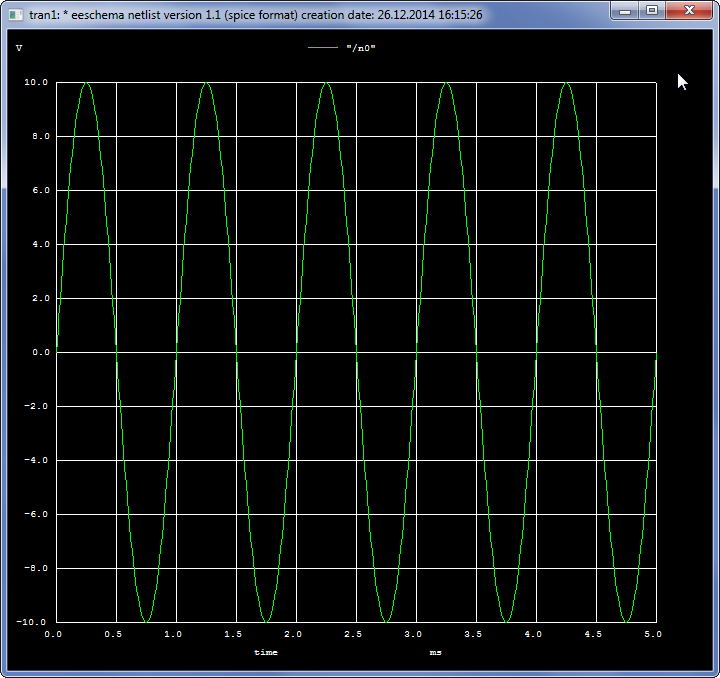
\includegraphics[height=\textheight]{spice/spice1.png}
\clearpage

Эта команда вывела напряжение при переходном процессе на цепи \net{n0}.

Как вы заметили, диаграмма сигнала отображается на черном фоне. Если вам нужны
другие цвета, например для вставки в документацию, их можно переопределить:

\begin{verbatim}
ngspice 12 -> set color0 = white
ngspice 13 -> set color1 = black
ngspice 14 -> set color2 = green
ngspice 3 -> plot "/n0"
\end{verbatim}

\noindent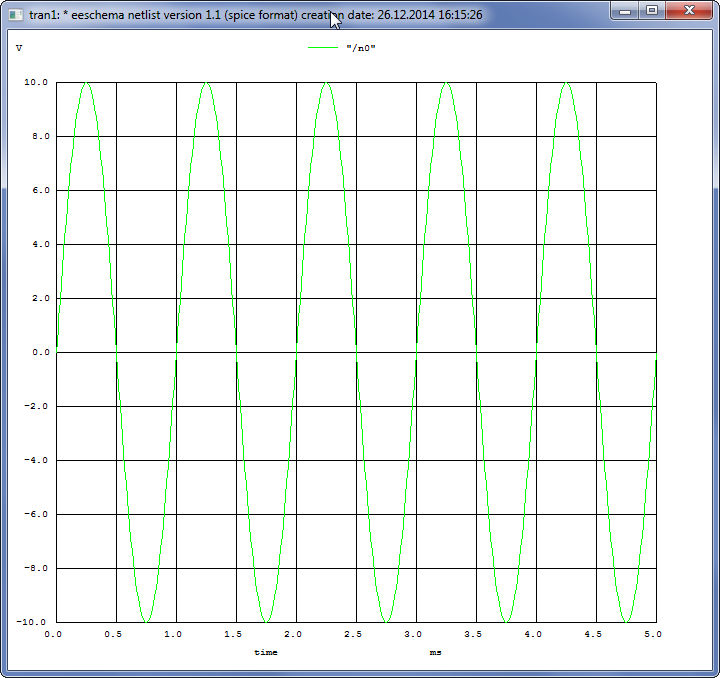
\includegraphics[height=0.5\textheight]{spice/spice2.png}

\bigskip
Диаграмма показывает форму входного сигнала, как мы и ожидали, но она нас мало
интересует, так как мы ее и задали. Нам интереснее например \emph{напряжение на
резисторе}, кроме того мы попробуем \emph{сравнить два сигнала}.
Это легко сделать указав два имени цепи:

\begin{verbatim}
ngspice 31 -> plot "/n0" "/n1"
\end{verbatim}

\clearpage
\noindent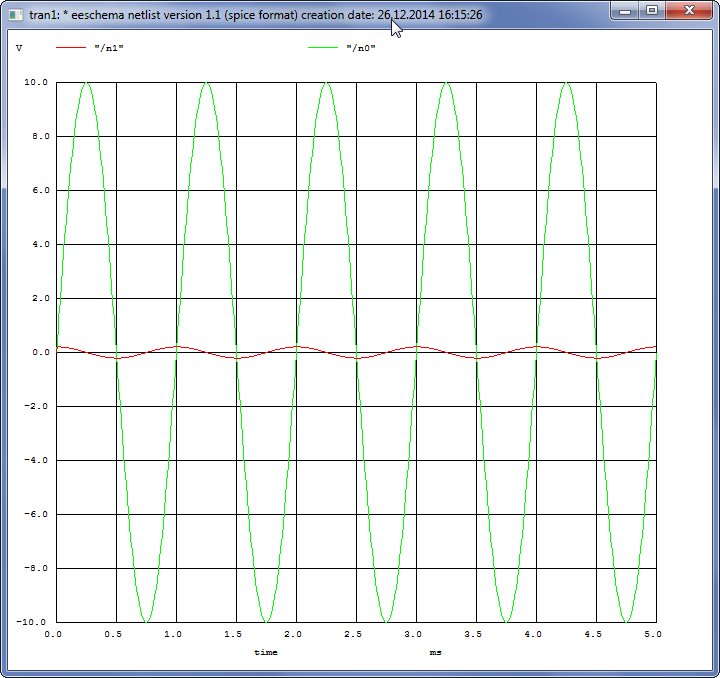
\includegraphics[height=\textheight]{spice/spice3.png}
\clearpage

\secrel{Расчет АЧХ по переменному току (AC симуляция)}

Сигнала на резисторе почти не видно. Теперь вопрос: какие частоты попускает наш
фильтр ? Для определения этого теперь выполним \term{расчет по переменному току
(AC симуляцию)}. Команда для этого \verb|ac ( DEC j OCT j LIN )N FStart FEnd|.

\verb|FStart| и \verb|FEnd|\ --- соответственно начальная и конечная частота.
Необязательные параметры \verb|DEC|, \verb|OCT| или \verb|LIN| указывают способ
изменения частоты: декадно, октавно или линейно. Если выборана октавная или
декадная \term{вариация частоты}, то параметр \verb|N| задает число
частот на декаду или октаву. Для выполнения \term{AC анализа} должен быть
изменен источни сигнала: сейчас он определен как синус с амплитудой 10\,В и
частотой 1\,КГц. Для анализа это должен быть \emph{источник переменного
апряжения}. Снова запускаем \eeschema\ и меняем значение источника:

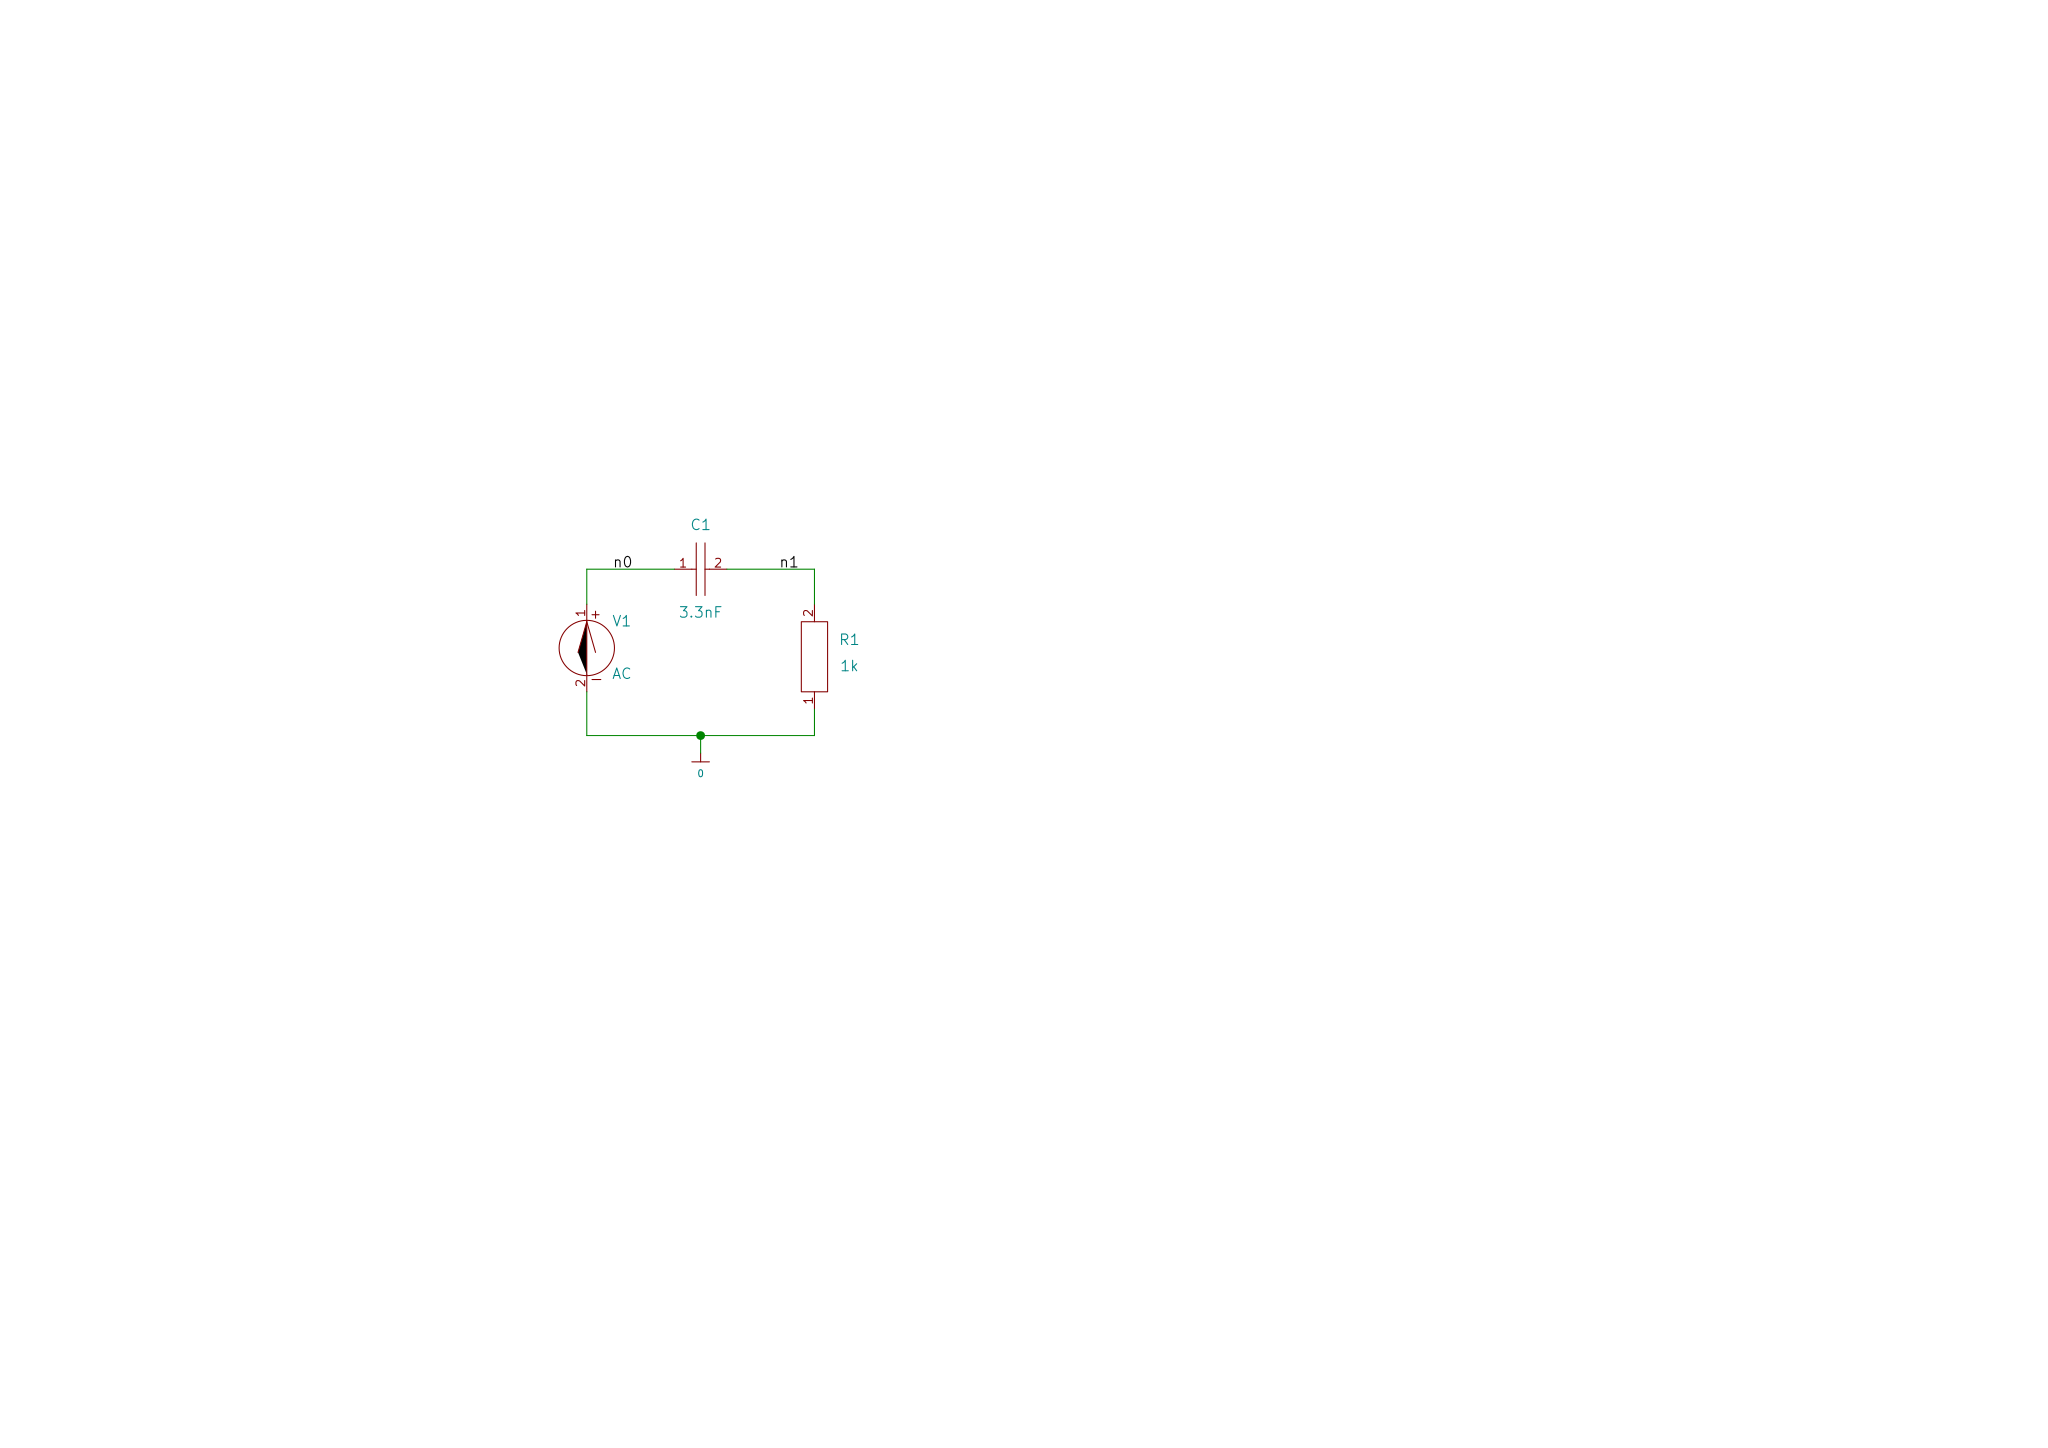
\includegraphics[height=0.5\textheight]{spice/ACanaliz.pdf}

Создаем нетлист, загружаем ео и запускаем команду AC анализа:

\begin{verbatim}
$ ngspice ACanaliz.cir
ngspice 1 -> ac lin 1000 0.1 250kHz
Doing analysis at TEMP = 27.000000 and TNOM = 27.000000

Warning: v1: has no value, DC 0 assumed


No. of Data Rows : 1000

ngspice 2 -> plot "/n1"
ngspice 3 -> plot "/n0" "/n1"
\end{verbatim}

Эта команда выполяняет \term{линейный AC анализ} от (почти) 0\,Гц до 250\,КГц.
Результат можно увидеть как напряжение для источника, так и напряжение на
\elem{R1}:

\pagebreak\noindent
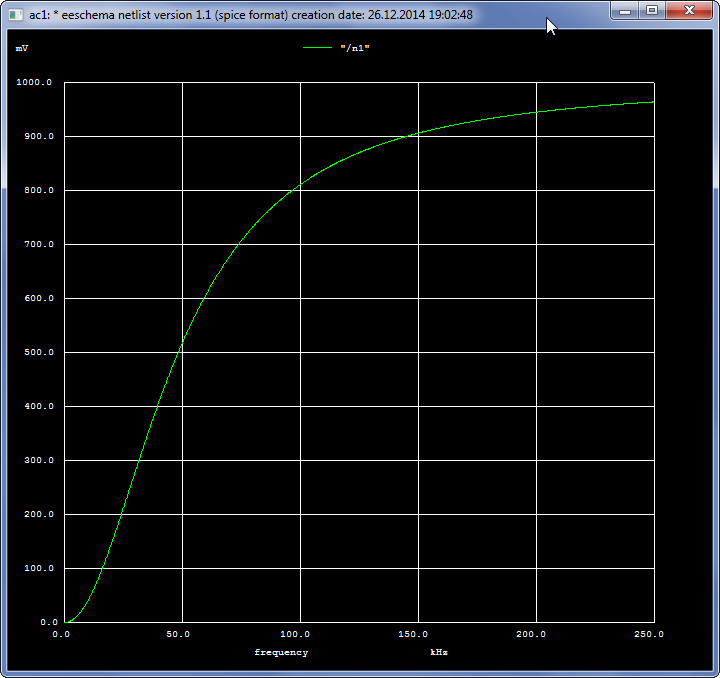
\includegraphics[height=\textheight]{spice/spice4.png}

\pagebreak\noindent
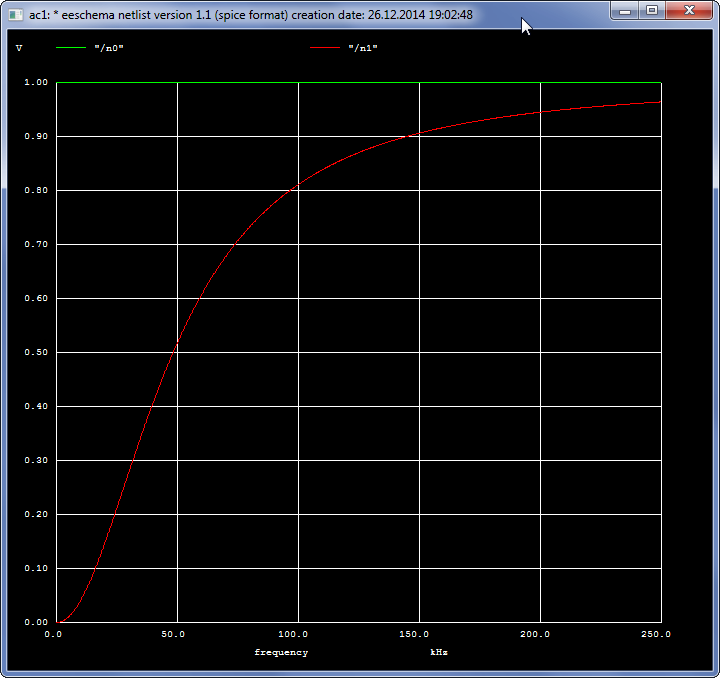
\includegraphics[height=\textheight]{spice/spice5.png}

\secrel{Симуляция полноволнового выпрямителя}

\noindent
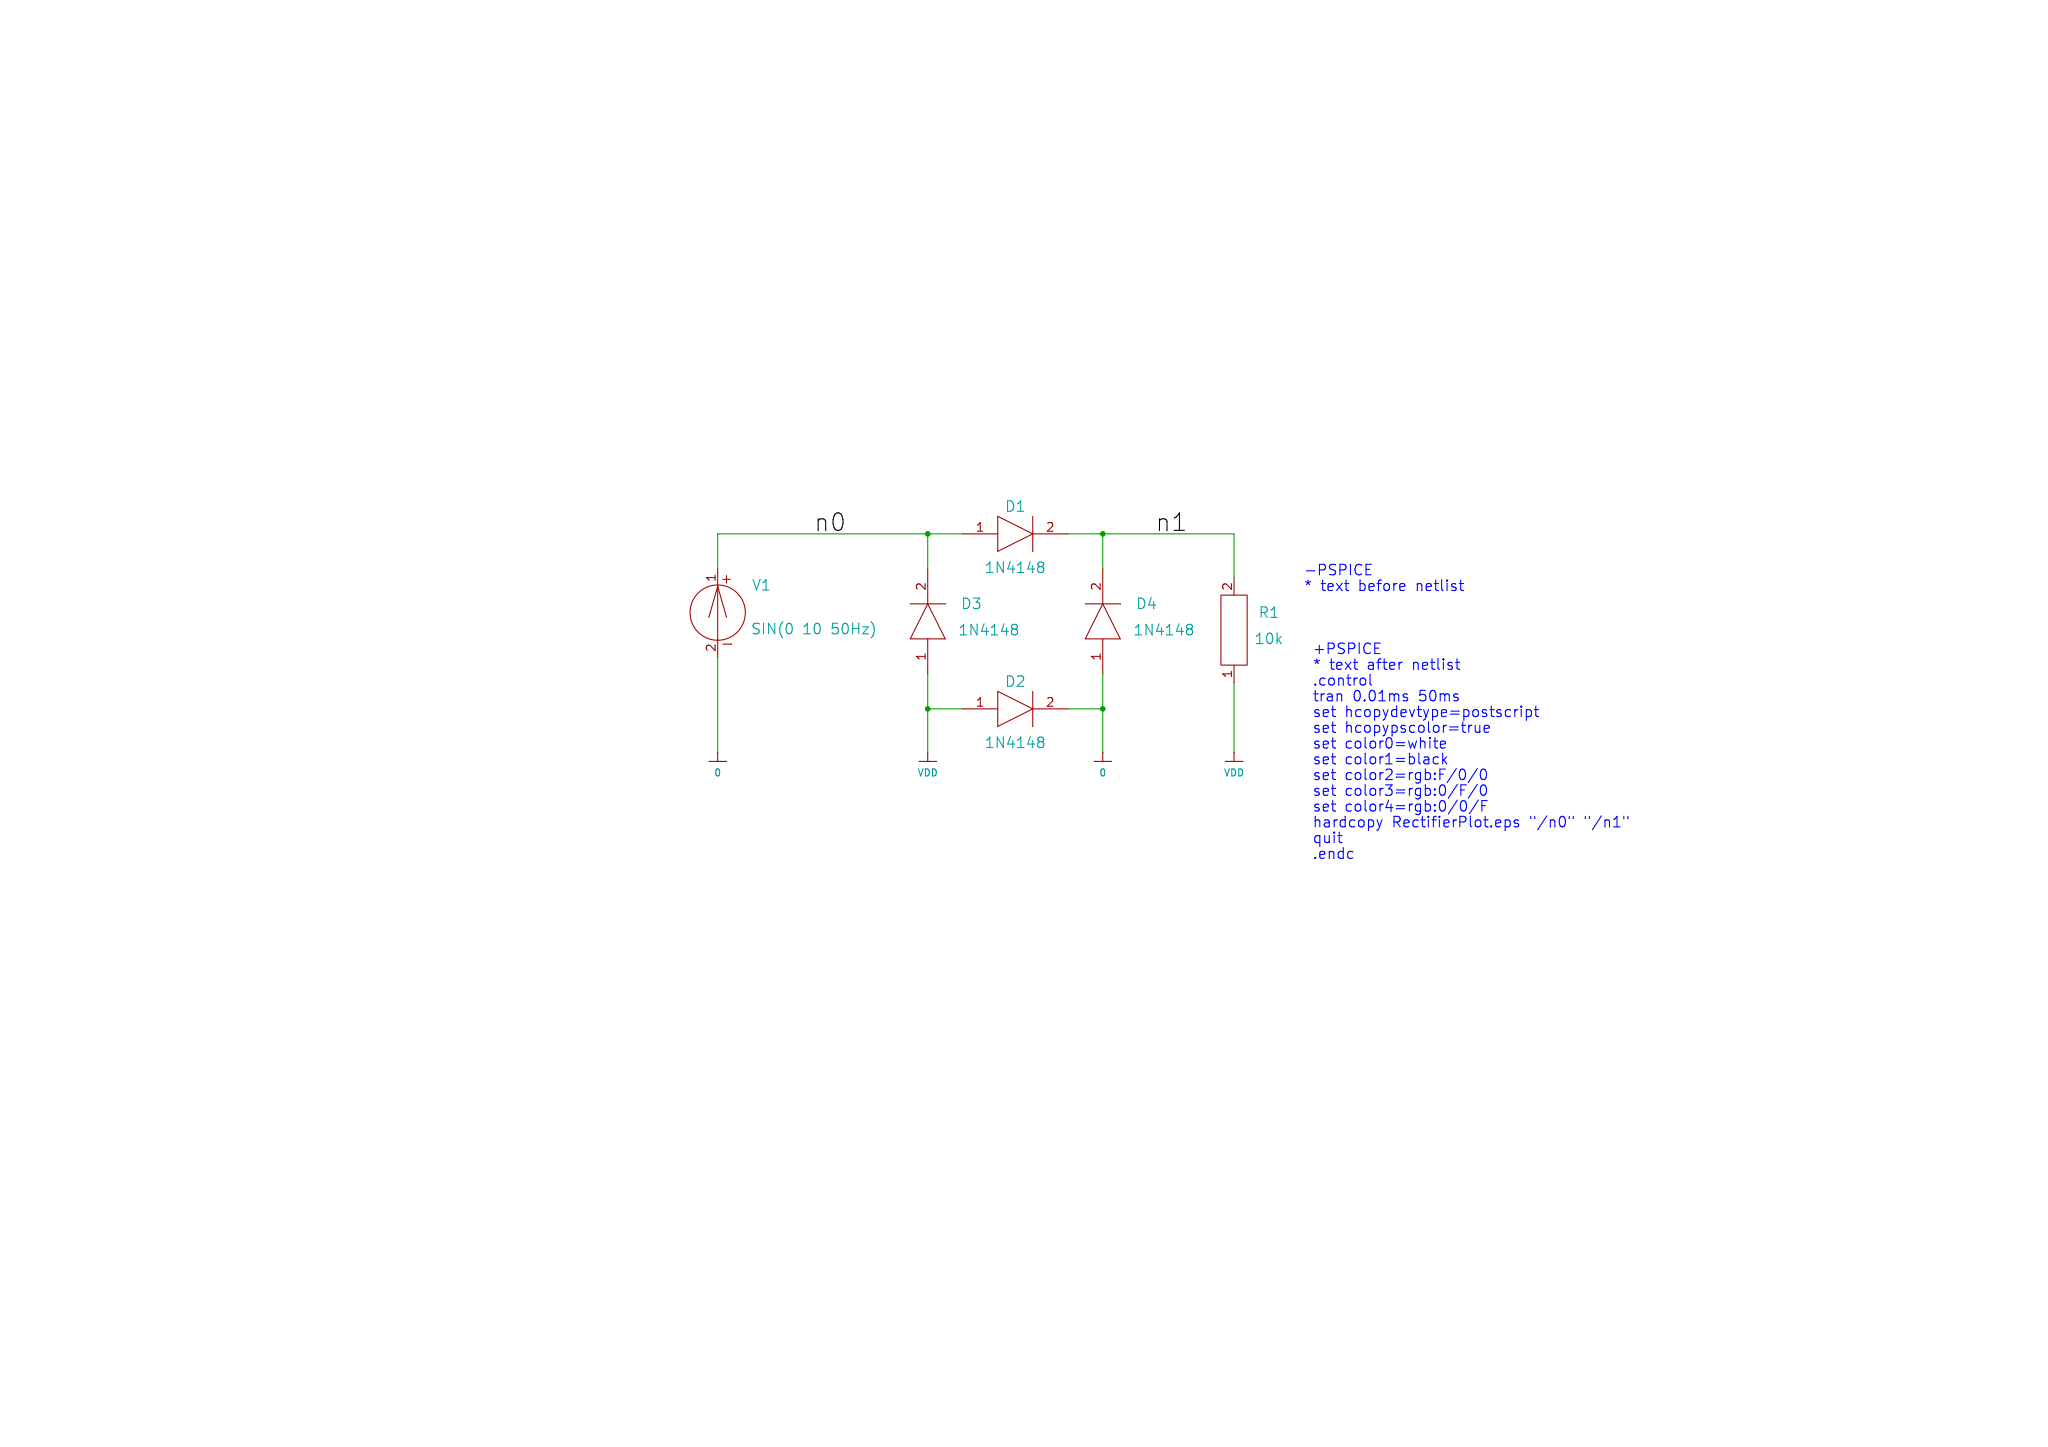
\includegraphics[height=0.5\textheight]{spice/Rectifier.pdf}

\lst{Rectifier.cir}{}{spice/Rectifier.cir}

\pagebreak\noindent
\includegraphics[height=\textheight]{spice/rectifierplot.eps}

% % In the following sections, we are going to simulate more circuits to get
% better involved with NG-spice.
% % 4 Simulating a full wave rectier
% % 1
% % +
% % 2
% % -
% % V1
% % SIN(0 10 50Hz)
% % D1
% % 1N4148
% % n0
% % R1
% % 10k
% % n1
% % 0
% % D2
% % 1N4148
% % D3
% % 1N4148
% % D4
% % 1N4148
% % Vdd Vdd
% % Figure 6: A full wave rectier.
% % Figure 6 shows the typical full wave rectier circuit. Both half waves of the input signal can be used, i.e.
% % the negative half wave is mirrored upwards. This can be seen in Figure 7 which shows the spice simulation of
% % the circuit.
% % time
% % 0.0 5.0 10.0 15.0 20.0 25.0 30.0 35.0 40.0 45.0 50.0
% % ms
% % -10.0
% % -5.0
% % 0.0
% % 5.0
% % 10.0
% % V v(n1,vdd) tran.v(n0)
% % Figure 7: Source voltage transient and voltage across R1
% % 
% % \secrel{Links to useful resources}
% % 
% % URLs
% % [1] , TBD <http://www.ecircuitcenter.com/>.
% % [2] , GPL Electronic Design Automation <http://geda.seul.org>.
% % [3] , TBD <gnucap> .
% % [4] , TBD <gwave> .
% % [5] , NG-SPICE: The free circuit simulator <http://www.ngspice.org>.

\secup
\secup
